\section{Verallgemeinerung von Klauseln}
\label{sec:ana:generalize}

Bisher erhaltene Klauseln werden in diesem Abschnitt darauf untersucht, ob eine Verallgemeinerung möglich ist. Verallgemeinerung bedeutet dabei, den Sinn der Klausel
zu erkennen und auf weitere Stellen anzuwenden. Auf Modulebene erfolgt dieser Prozess bereits automatisch, da diese Klauseln überall dort angewendet werden, wo das
Modul zum Einsatz kommt. Eine weitere Möglichkeit ist es, weitere Stellen innerhalb des Moduls zu identifizieren, an denen die Klausel ebenfalls gültig ist. Besonders
gut funktioniert diese Verallgemeinerung bei dem Addierer. Durch die Breite von 32 Bit können viele Klauseln bitweise nach vorne oder hinten verschoben werden und sind
an diesen Stellen ebenfalls gültig. Aufgrund der Vielzahl der erhaltenen Klauseln ist jedoch eine weitere Unterteilung notwendig. Zunächst werden die in Abschnitt
\ref{sec:knf:addierer} erläuterten Komponenten des Addierers (Halb-, Voll- und Mod-2 Addierer) in eigene Module mit dem Level eins ausgelagert. Dadurch können viele
Klauseln direkt den Halb-, Voll und Mod-2 Addiereren zugeordnet werden. Ein Großteil der erworbenen Klauseln verbleibt aber nach wie vor im Modul des 32-Bit Addierers.
Bei der Analyse der verbleibenden Klauseln zeigt sich, dass sich diese Klauseln in Halb-, Voll und Mod-2 Addiereren höherer Ebene organisieren lassen. Als Addierer
höherer Ebene wird ein Addierer bezeichnet, der bei Bedarf ein eingehendes oder ausgehendes Carrybit berücksichtigt, intern jedoch keine Carrybits verwendet. Diese
Addierer entsprechen dem Carry-Lookahead Addierer (siehe Abschnitt \ref{sec:grundlagen_add}) in unterschiedlichen Bitbreiten. Ergänzt werden Module für Addierer bis
vier Bit Breite. Abbildung \ref{fig:sha256_module_add} zeigt die Erweiterung der Modulhierarchie.
\begin{figure}[!h]
  \centering
  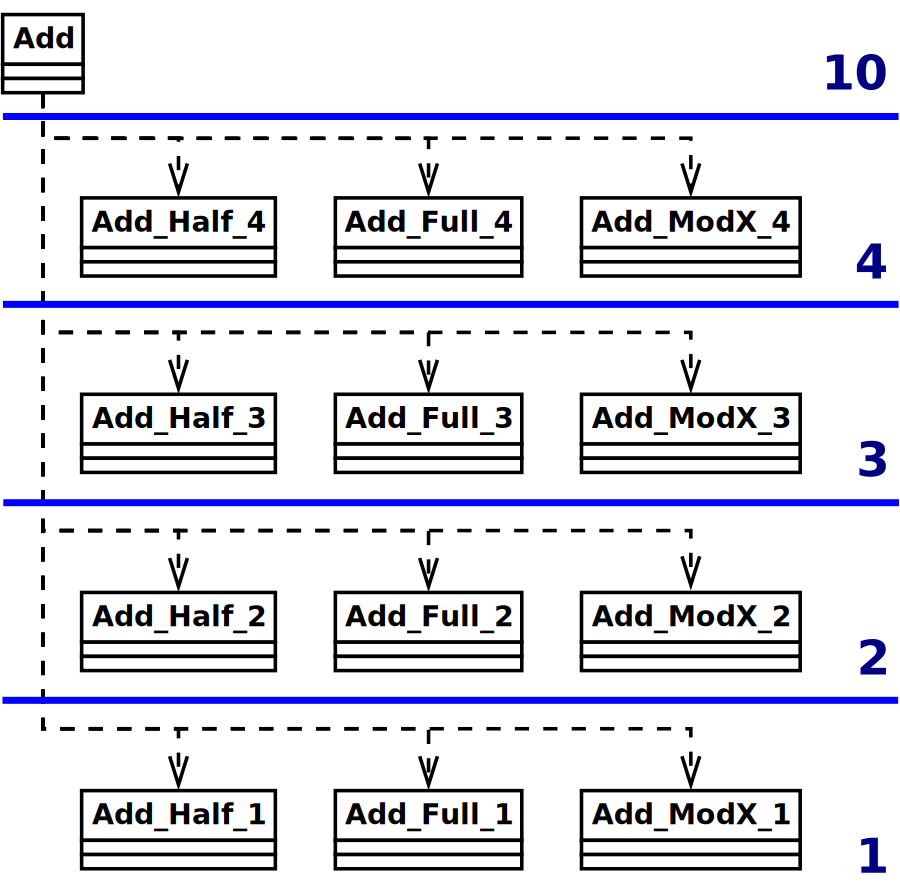
\includegraphics[scale=0.265]{images/module_add}
  \caption{Ergänzte Module von \glos{sha256}}
  \label{fig:sha256_module_add}
\end{figure}

Module für Addierer mit mehr als vier Bit Breite werden nicht ergänzt, da der SAT-Solver keine Klauseln ermittelt hat, die diesen Modulen zugeordnet werden könnten.  
Notwendig für die Funktion des Addierers sind nur die Module mit dem Level eins. Die Module mit dem Level zwei bis vier dienen als zusätzliche Information
auf den selben Literalen. Durch dieses Vorgehen erfolgt die Verallgemeinerung von Klauseln innerhalb des Addierers ebenfalls automatisch.

Bei den anderen Modulen zeigt sich kein Muster dieser Art und die Anzahl der erworbenen Klauseln ist vergleichsweise gering. Deshalb werden die erworbene Klauseln
darin direkt untergebracht und durch Verwendung einer Schleife verallgemeinert in sofern dies möglich ist. Eine Ausnahme bildet das Modul der vollständigen
Kompressionsfunktion. Neben der Verallgemeinerung auf Bitbreite bietet sich in diesem Modul die Möglichkeit, die Klauseln auch auf weitere Runden anzuwenden.
Klauseln die sich nur auf eine Runde beziehen wurden schon dem Modul für die Rundenfunktion zugeordnet, so dass nur noch Klauseln betrachtet werden die sich über
zwei oder mehr Runden erstrecken. Jedes Literal der jeweiligen Klausel wird dann um eine Runde nach vorne oder hinten verschoben.

Beachtet werden muss jedoch, dass jede der 64 Runden eine andere Rundenkonstante verwendet und die Erweiterung der Eingabe bei den ersten 16 Runden keine
Anwendung findet. Während bei den anderen Modulen im Allgemeinen eine Verallgemeinerung entweder funktioniert oder nicht, muss dadurch jede durch die
Verallgemeinerung generierte Klausel einzeln überprüft werden. Wie auch bei der Überprüfung der modulspezifischen Klauseln in Abschnitt \ref{sec:ana:module}
wird das Programm "`clausechecker"' für die Überprüfung genutzt. Nur wenige der ermittelten Klauseln lassen sich ohne Einschränkungen auf weitere Bits oder
Runden übertragen. Der clausechecker generiert deshalb ein zweidimensionales Array, in dem die gültigen Klauseln markiert werden. Dieses Array wird dann im
Modul der Kompressionsfunktion genutzt, um die gültigen Klauseln zu generieren.

\TODO{bezug zu konstanten erklären}